\chapter{Appendices} % * means unnumbered heading
%\addcontentsline{toc}{chapter}{Appendices} % add to table of contents although not a numbered heading
\label{c:Appendices}

\section{Datasets in differential cross section analysis}
\label{as:datasets}

\begin{table}[hbth]
\centering
\begin{tabular}{llrr}
\hline
\textbf{Data set name} & \textbf{Run period} & \textbf{$\mathbf{L_{int}}$ / \pbinv} & \textbf{Runs} \\
\hline
ElectronHad 12 Oct 2013 ReReco & Run2011A & 2,333 & 160404--173692 \\
ElectronHad 12 Oct 2013 ReReco & Run2011B & 2,738 & 175833--180252 \\
\hline
SingleMu 12 Oct 2013 ReReco & Run2011A & 2,331 & 160404--173692 \\
SingleMu 12 Oct 2013 ReReco & Run2011B & 2,766 & 175833--180252 \\
\hline
\end{tabular}
\caption{7 TeV data sets by run period with the corresponding integrated
luminosities ($L_{int}$) and run numbers.}
\label{tab:datasets7TeV}
\end{table}

\begin{table}[hbth]
\centering
\begin{tabular}{llrr}
\hline
\textbf{Data set name} & \textbf{Run period} & \textbf{$\mathbf{L_{int}}$ / \pbinv} & \textbf{Runs} \\
\hline
SingleElectron 22 Jan 2013 ReReco & Run2012A & $883.3$ & 190456--193621 \\
SingleElectron 22 Jan 2013 ReReco & Run2012B & $4,389.0$ & 193834--196531 \\
SingleElectron 22 Jan 2013 ReReco & Run2012C & $7,137.0$ & 198022--203742 \\
SingleElectron 22 Jan 2013 ReReco & Run2012D & $7,318.0$ & 203777--208686 \\
\hline
SingleMu 22 Jan 2013 ReReco & Run2012A & $889.4$ & 190456--193621 \\
SingleMu 22 Jan 2013 ReReco & Run2012B & $4,424.0$ & 193834--196531 \\
SingleMu 22 Jan 2013 ReReco & Run2012C & $7,152.0$ & 198022--203742 \\
SingleMu 22 Jan 2013 ReReco & Run2012D & $7,280.0$ & 203777--208686 \\
\hline
\end{tabular}
\caption{8 TeV data sets by run period with the corresponding integrated
luminosities ($L_{int}$) and run numbers.}
\label{tab:datasets8TeV}
\end{table}

\begin{table}[hbth]
\centering
\begin{tabular}{lr}
\hline
\textbf{Data Period} & \textbf{Mask} \\
\hline
2011 & \verb|Cert_160404-180252_7TeV_ReRecoNov08_Collisions11_JSON_v2.txt| \\
2012 & \verb|Cert_190456-208686_8TeV_22Jan2013ReReco_Collisions12_JSON.txt| \\
\hline
\end{tabular}
\caption{JSON files used for the 2011 and 2012 data taking periods.}
\label{tab:JSONfiles}
\end{table}

\section{Data-MonteCarlo corrections}
\label{as:data_monte_carlo_corrections}
\begin{figure}[hbtp]
    \centering
      \includegraphics[width=0.48\textwidth]{Chapters/04_Analysis/04b_XSections/images/control_plots/before_fit/7TeV/EPlusJets_nVertex__with_ratio}\hfill
      \includegraphics[width=0.48\textwidth]{Chapters/04_Analysis/04b_XSections/images/control_plots/before_fit/7TeV/EPlusJets_nVertex_reweighted__with_ratio}\\
      \includegraphics[width=0.48\textwidth]{Chapters/04_Analysis/04b_XSections/images/control_plots/before_fit/8TeV/EPlusJets_nVertex__with_ratio}\hfill
      \includegraphics[width=0.48\textwidth]{Chapters/04_Analysis/04b_XSections/images/control_plots/before_fit/8TeV/EPlusJets_nVertex_reweighted__with_ratio}\\
     \caption{Distributions of the number of reconstructed vertices in an event in the muon+jets
     channel before implementing pileup reweighting (left) and after implementation (right) at $\roots=7\TeV$
     (upper) and $\roots=8\TeV$ (lower).}
     \label{fig:nvertices_before_and_after_pileup_reweighting_muons}
\end{figure}

\begin{figure}[hbtp]
    \centering
      \includegraphics[width=0.48\textwidth]{Chapters/04_Analysis/04b_XSections/images/control_plots/before_fit/7TeV/MuPlusJets_N_BJets_with_ratio}\hfill
      \includegraphics[width=0.48\textwidth]{Chapters/04_Analysis/04b_XSections/images/control_plots/before_fit/7TeV/MuPlusJets_N_BJets_reweighted_with_ratio}\\
      \includegraphics[width=0.48\textwidth]{Chapters/04_Analysis/04b_XSections/images/control_plots/before_fit/8TeV/MuPlusJets_N_BJets_with_ratio}\hfill
      \includegraphics[width=0.48\textwidth]{Chapters/04_Analysis/04b_XSections/images/control_plots/before_fit/8TeV/MuPlusJets_N_BJets_reweighted_with_ratio}\\
     \caption{Distributions of the number of \btags in an event in the muon+jets channel before applying
     \btag scale factors (left) and after application (right) at $\roots=7\TeV$
     (upper) and $\roots=8\TeV$ (lower).}
     \label{fig:nbjets_before_and_after_btag_scale_factors_muons}
\end{figure}

\begin{figure}[hbtp]
    \centering
      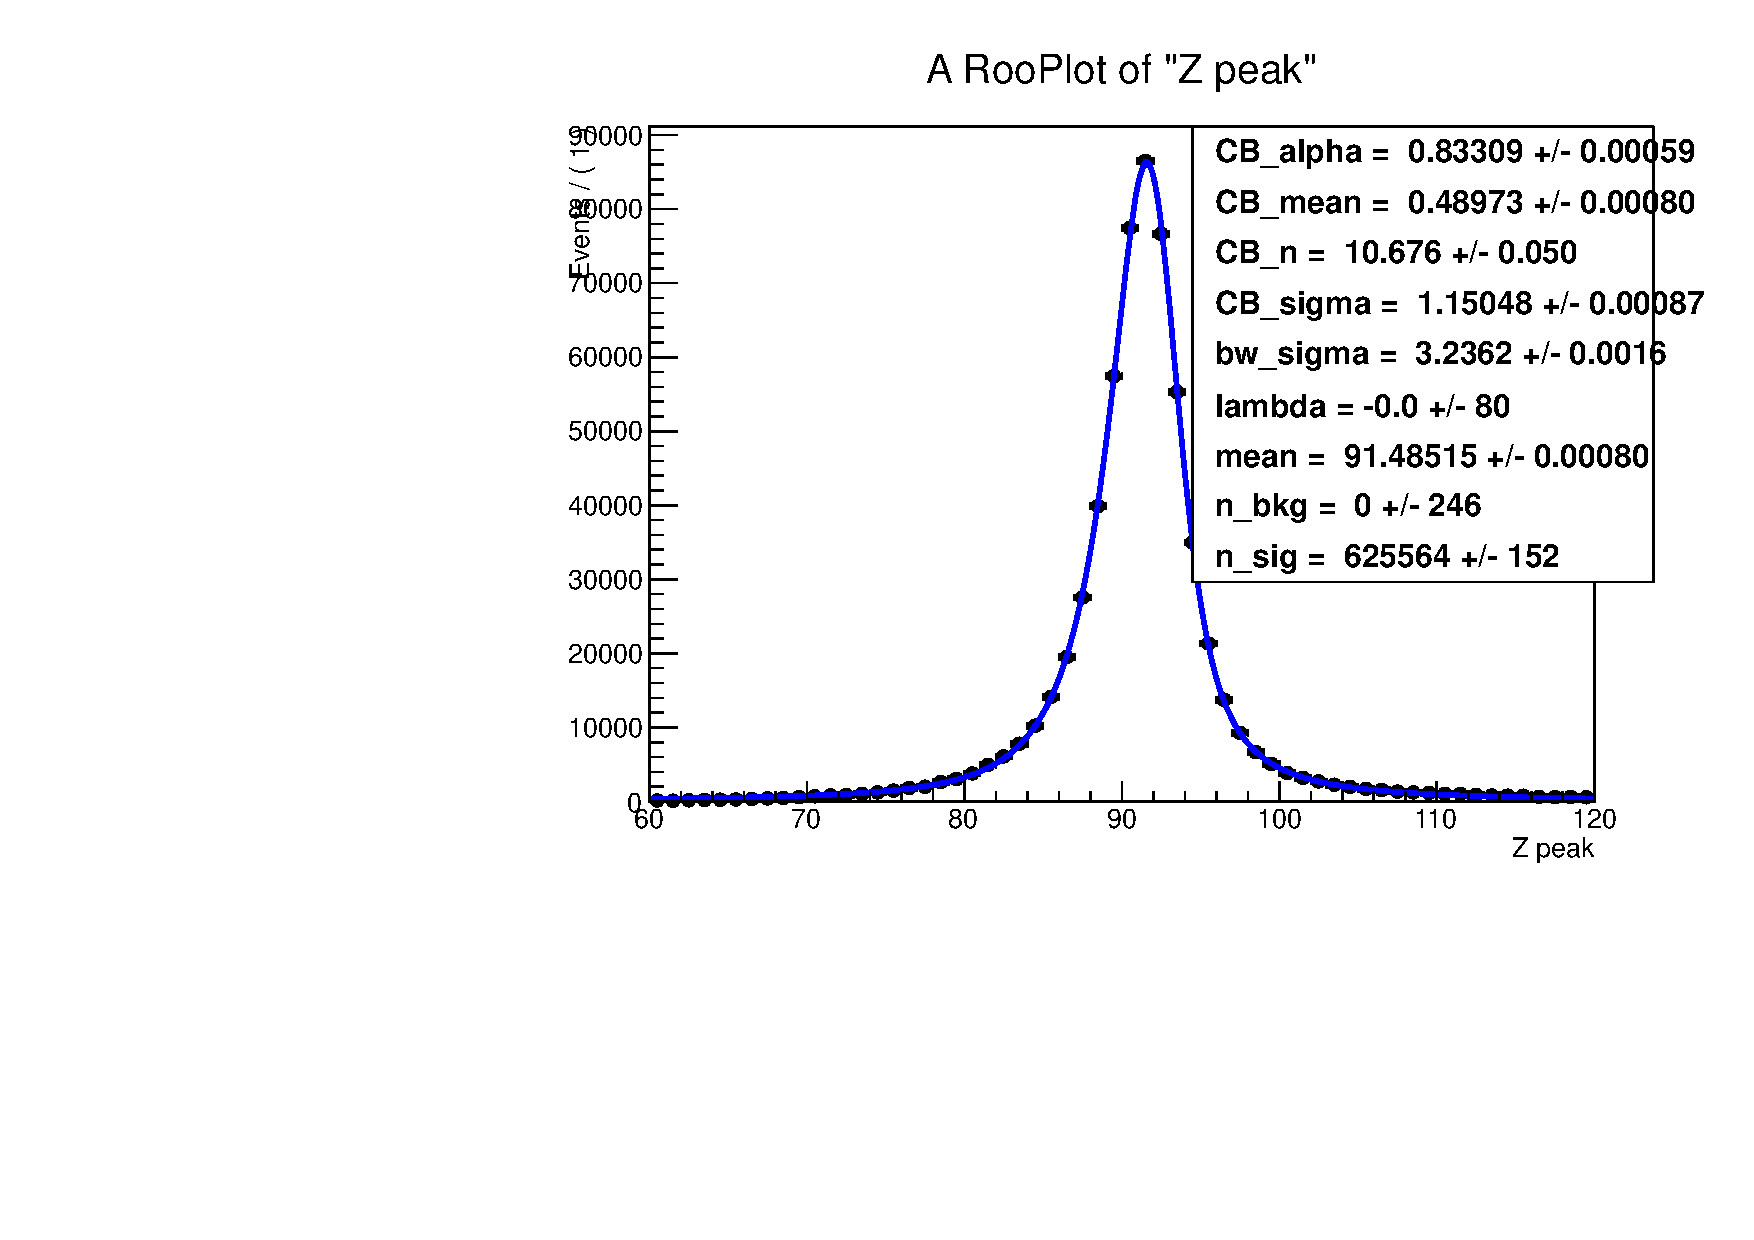
\includegraphics[width=0.48\textwidth]{Chapters/04_Analysis/04b_XSections/images/lepton_scale_factors/CBConvolution/electron/data/trigger/tagProbe_total_Z_peak}\hfill
      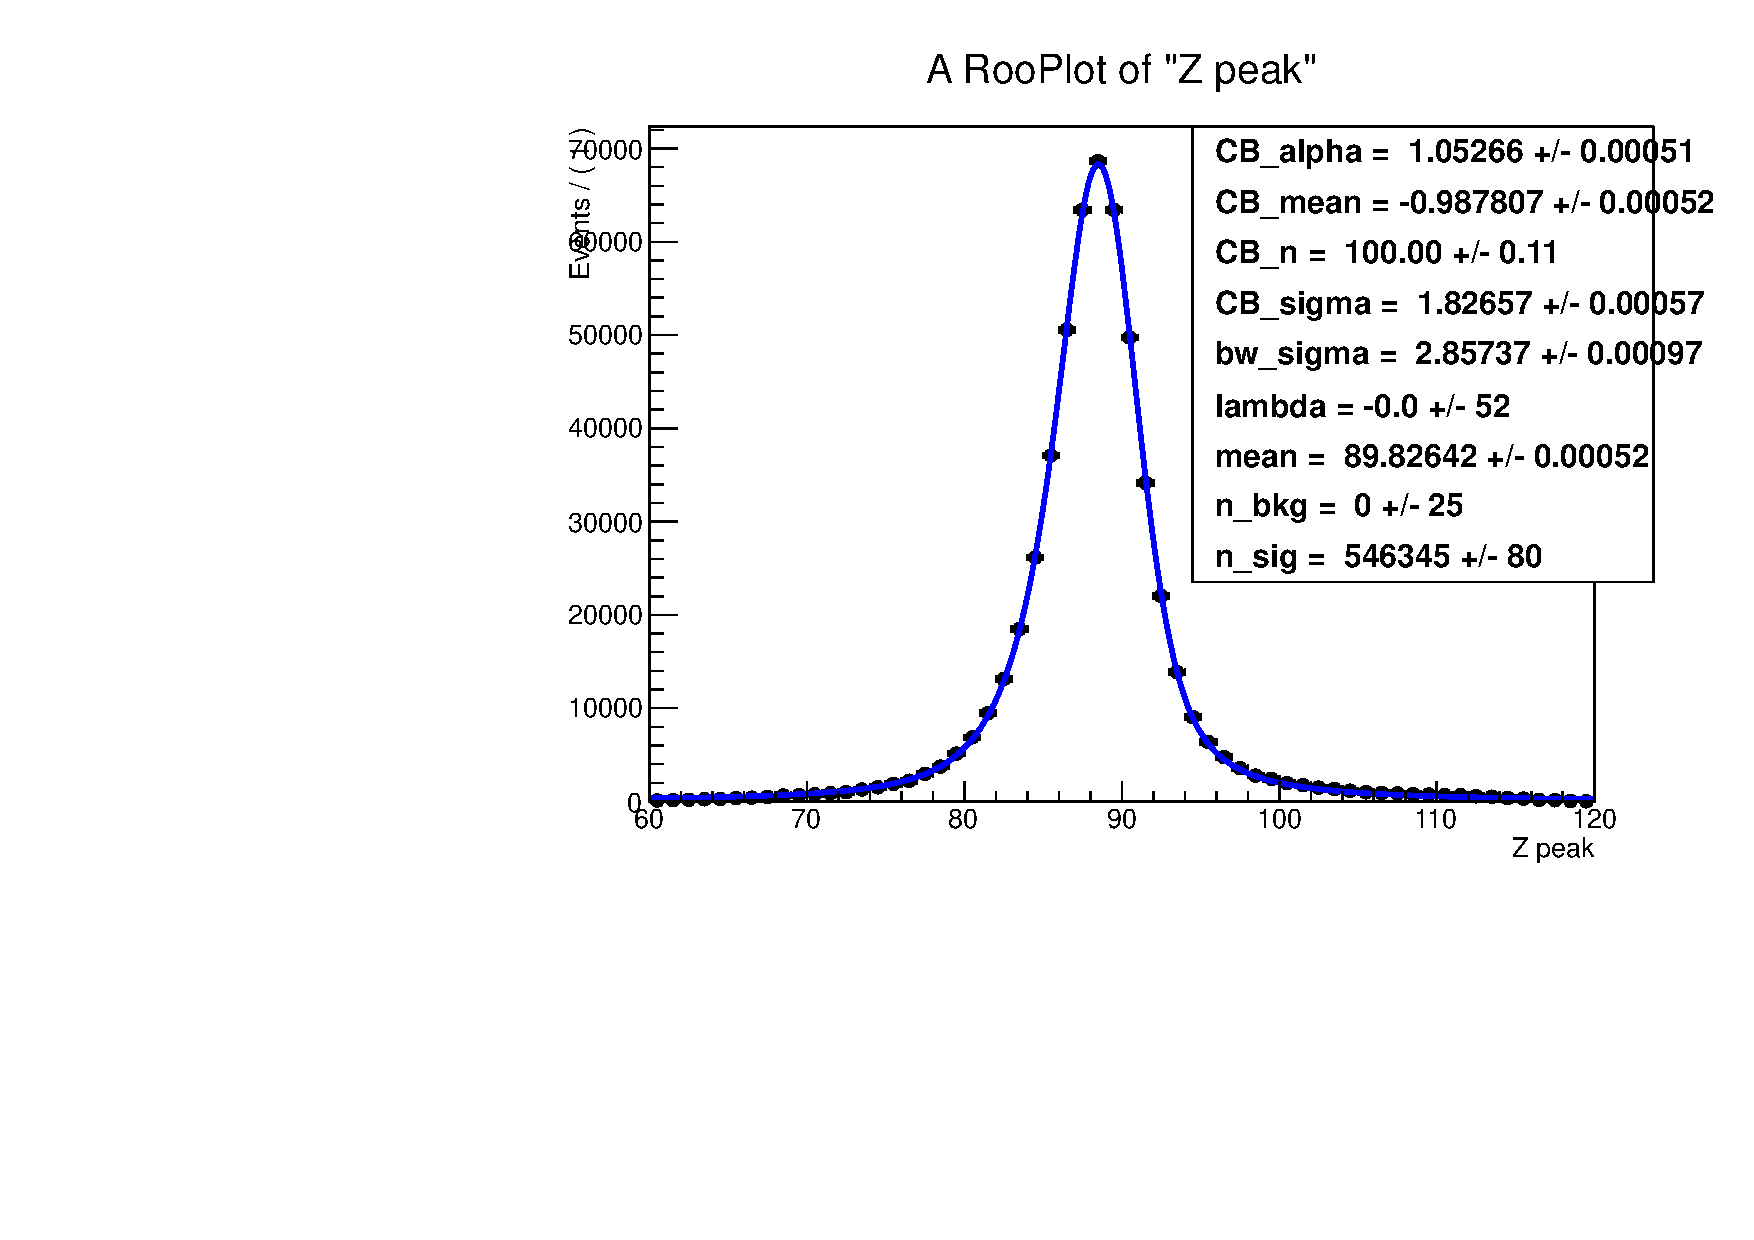
\includegraphics[width=0.48\textwidth]{Chapters/04_Analysis/04b_XSections/images/lepton_scale_factors/CBConvolution/electron/data/trigger/tagProbe_passed_hlt_Z_peak}\\
     \caption{Fits of the invariant mass distribution of all tag-and-probe pairs (left) and for
     tag-and-probe pairs in which the probe passes the trigger (right).}
     \label{fig:electron_trigger_efficiency_invariant_Z_mass_fits}
\end{figure}

\begin{figure}[hbtp]
    \centering
      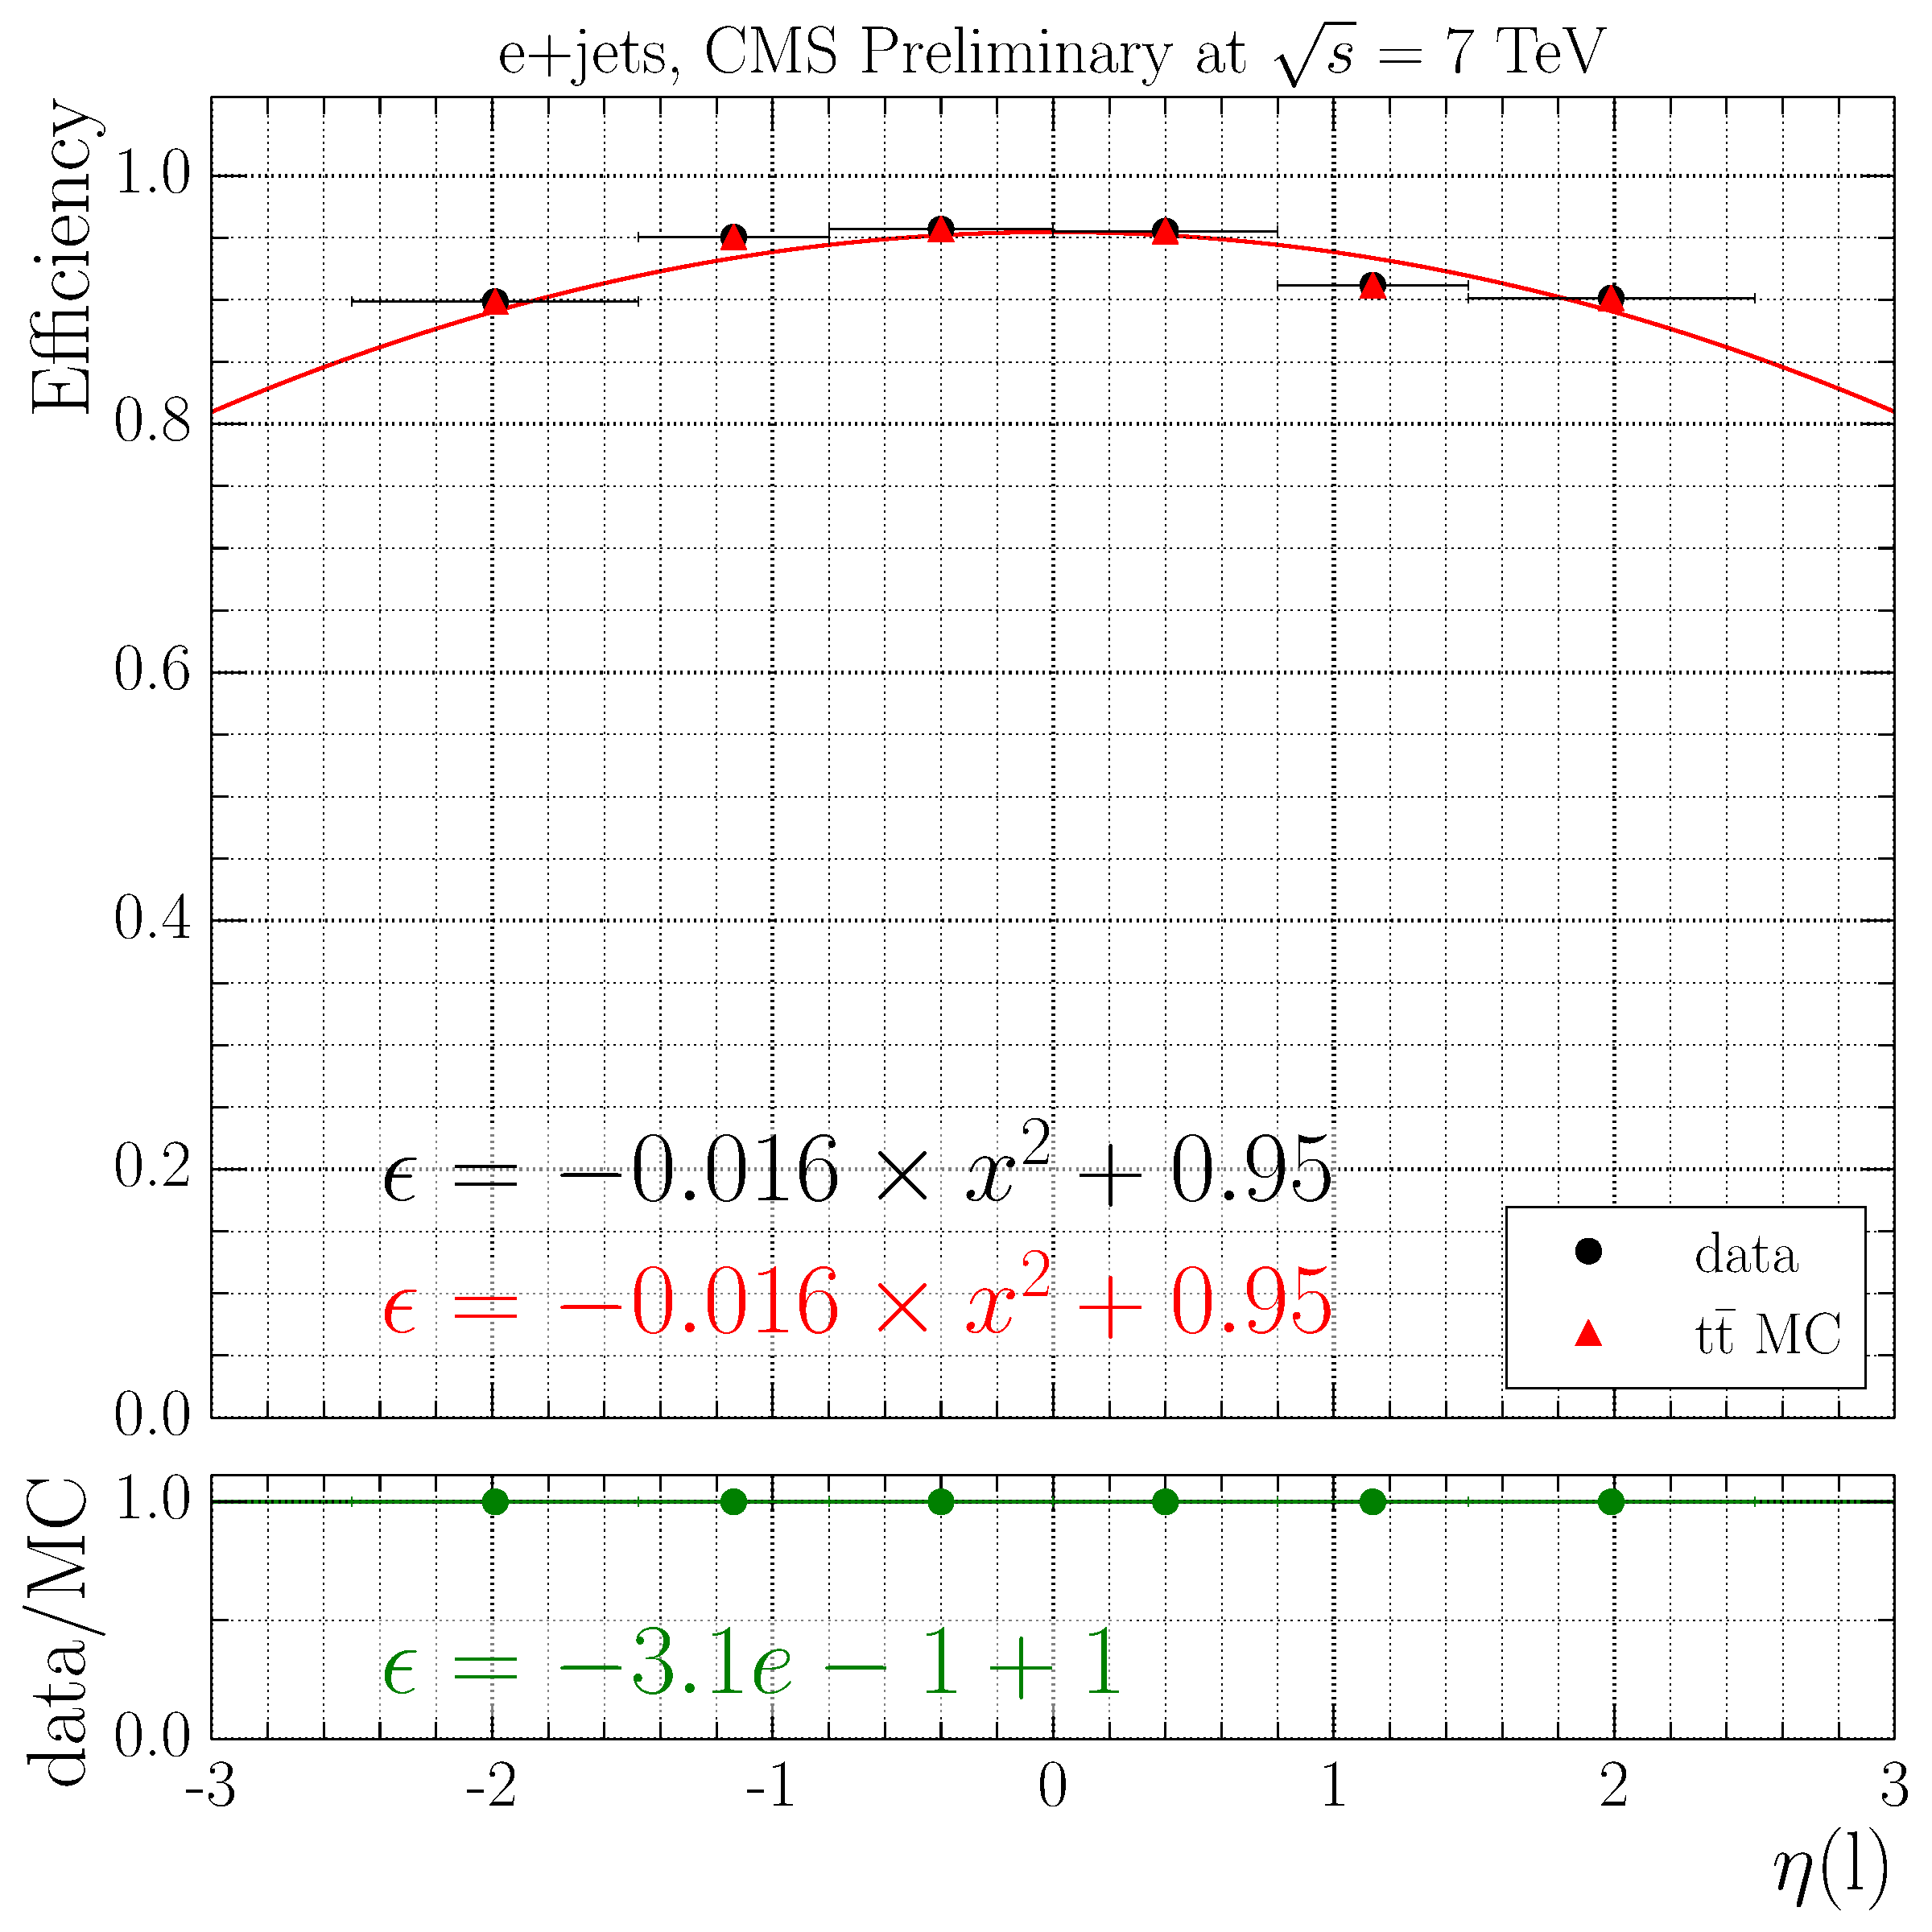
\includegraphics[width=0.48\textwidth]{Chapters/04_Analysis/04b_XSections/images/lepton_scale_factors/CBConvolution/electron/efficiency_eta_trigger}\hfill
      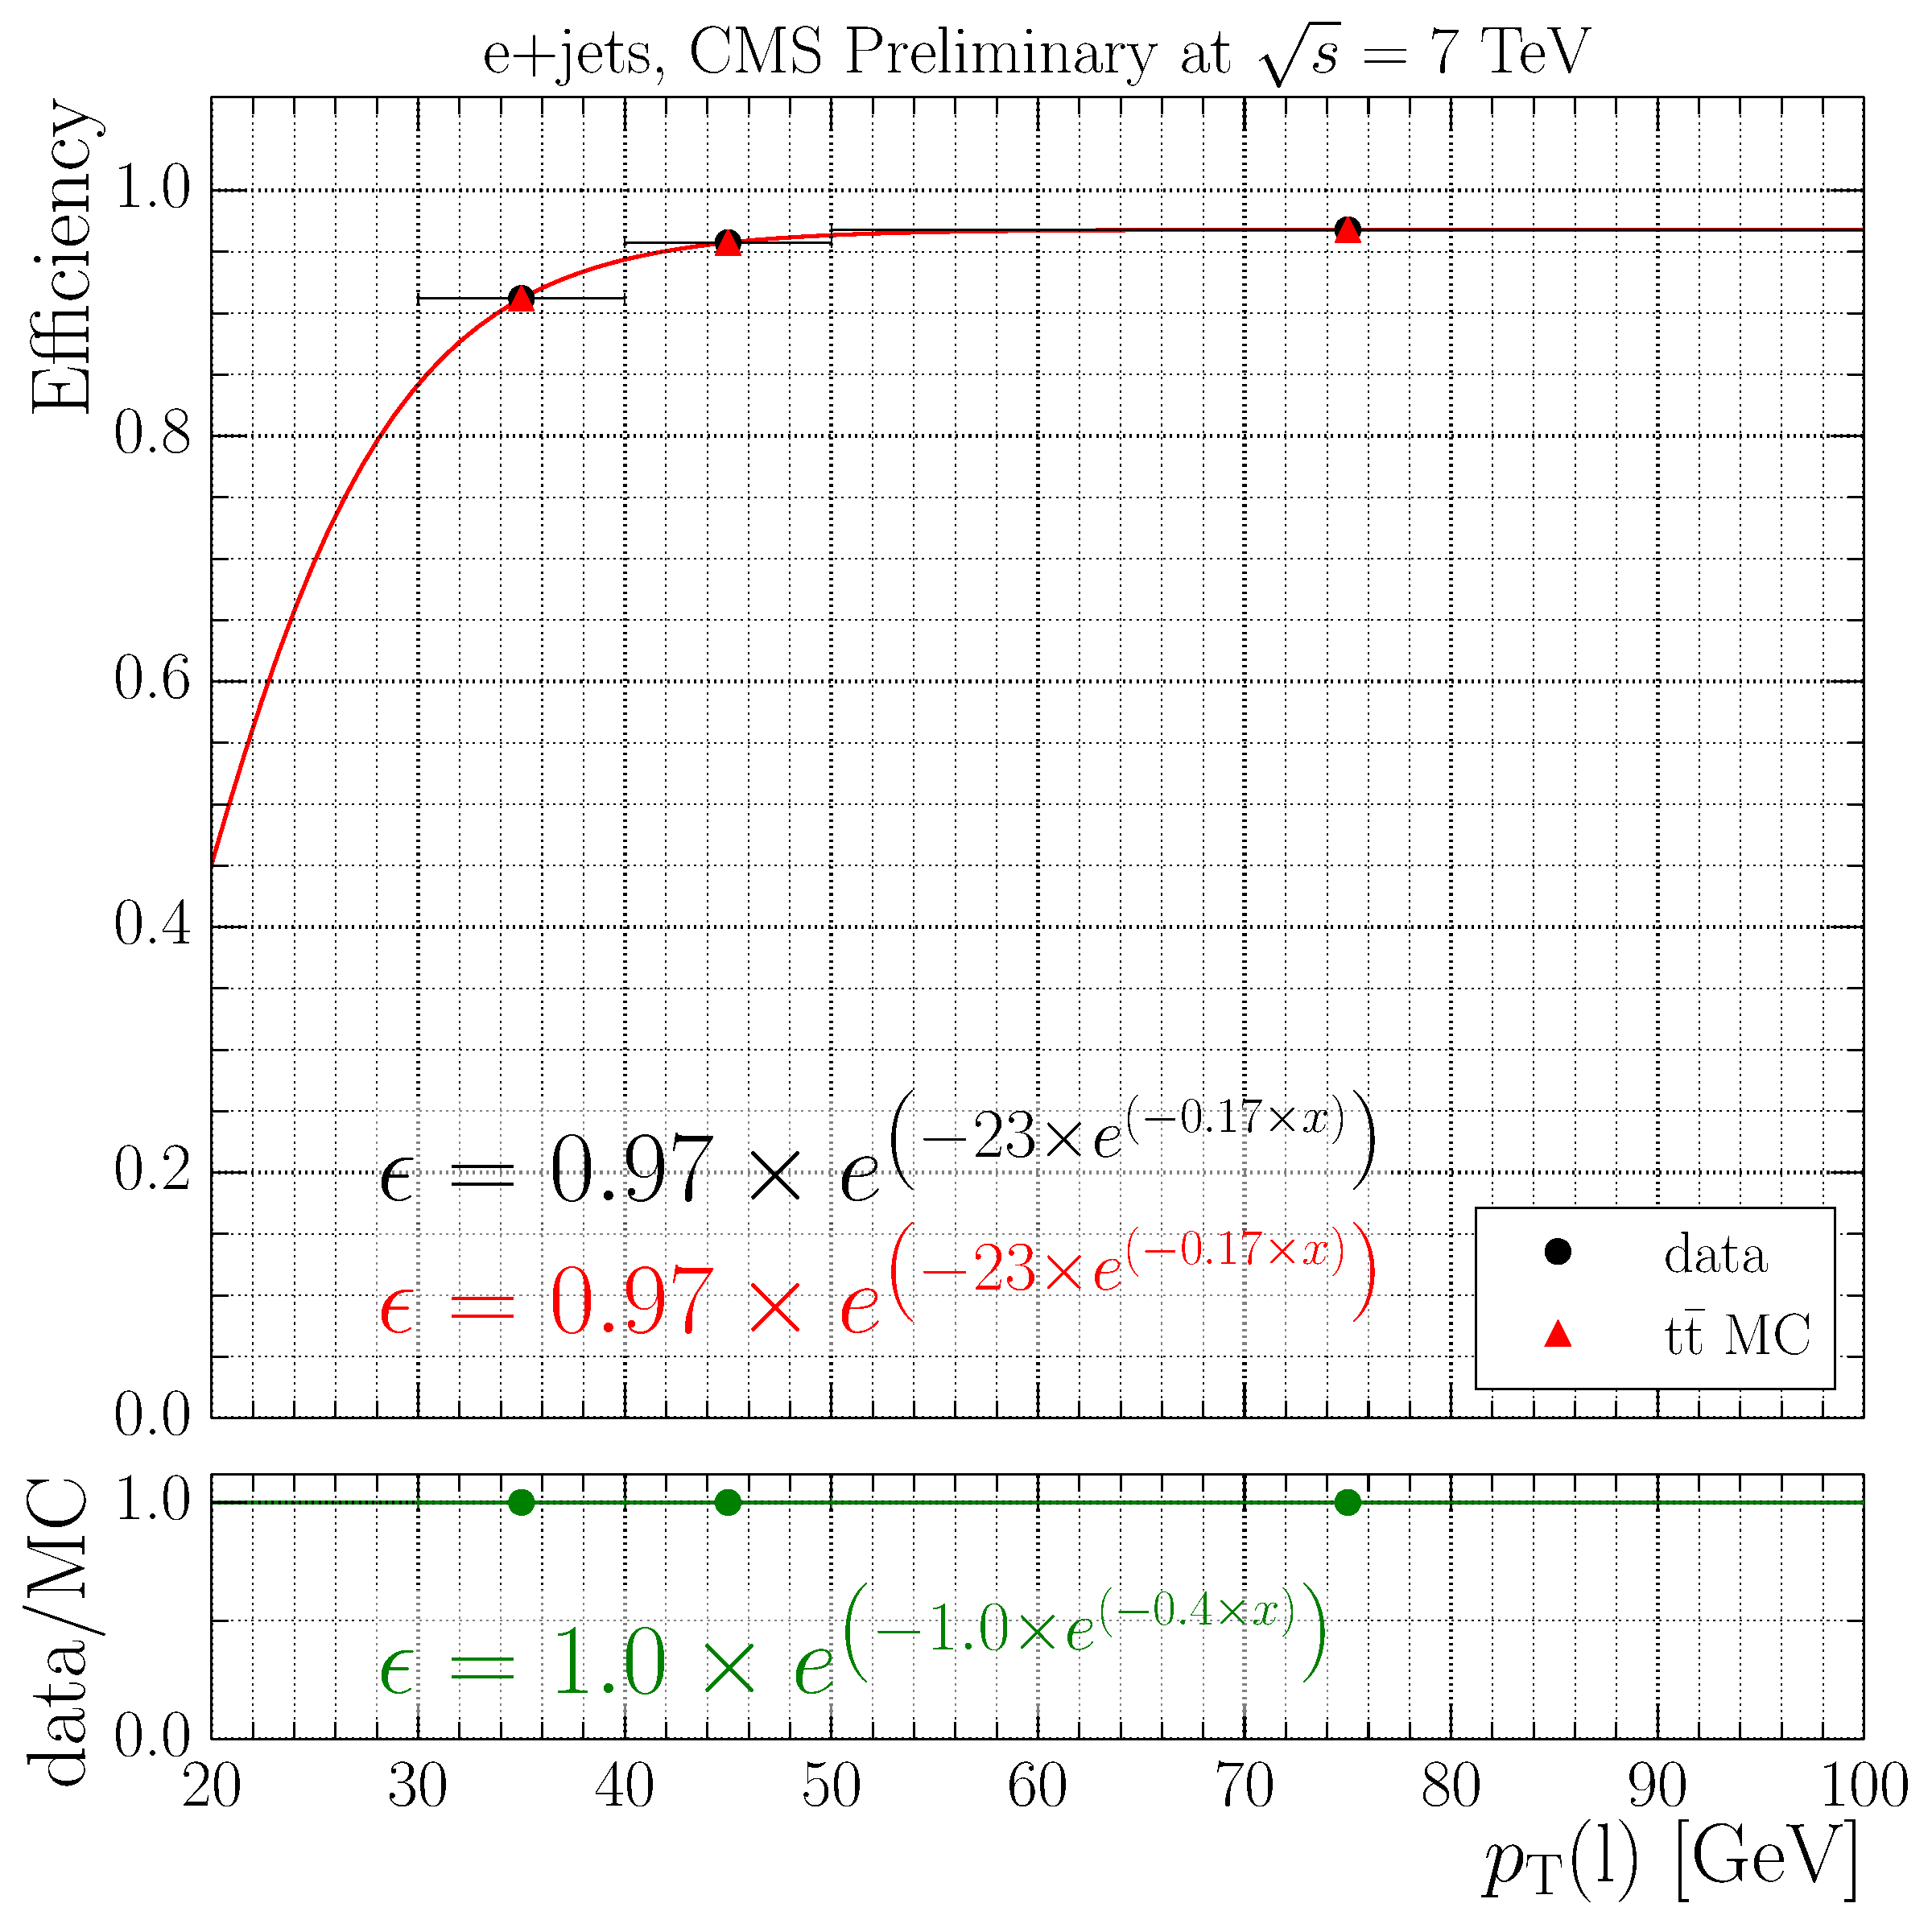
\includegraphics[width=0.48\textwidth]{Chapters/04_Analysis/04b_XSections/images/lepton_scale_factors/CBConvolution/electron/efficiency_pt_trigger}\hfill
      \caption{Trigger efficiencies as a function of $\eta$ and \pt in data and \ttbar Monte Carlo
      simulation.}
     \label{fig:electron_trigger_efficiencies_wrt_eta_pt}
\end{figure}
